% !TeX program = XeLaTeX
\documentclass[a4paper,oneside,12pt]{report}

% بسته‌های اولیه
\usepackage[top=30mm, bottom=30mm, left=30mm, right=30mm]{geometry}
\usepackage{amsmath,amsthm,amssymb,mathtools}
\usepackage{graphicx}
\usepackage{booktabs}
\usepackage{longtable}
\usepackage{setspace}
\usepackage{algorithm}
\usepackage{algorithmic}
\usepackage{listings}
\usepackage[table]{xcolor}
\usepackage{subcaption}
\usepackage{float}
\usepackage{multirow}
\usepackage{array}
\usepackage{threeparttable}
\usepackage{url}
\usepackage{indentfirst}
\usepackage{tocloft}
\usepackage{emptypage}
\usepackage{titlesec}
\usepackage{xspace}
\usepackage{bidipoem}
\usepackage[textfont={small},labelfont={rm,small},format=hang,labelsep=quad,justification={centering},aboveskip=1pt,belowskip=1pt]{caption}
\usepackage[nottoc,notlof,notlot]{tocbibind}
\usepackage{appendix}
\usepackage{lscape}
\usepackage{courier}
\usepackage[most, breakable]{tcolorbox}

% بسته bibliography با biber
\usepackage[backend=biber,style=numeric,sorting=none]{biblatex}
\addbibresource{MAGNET_Complete_Paper_Copy.bib}
% نمایش تمام مراجع (حتی آن‌هایی که استفاده نشده‌اند)
\ExecuteBibliographyOptions{uniquename=false,uniquelist=false}
\nocite{*}

% تنظیمات رنگ‌ها
\definecolor{Blue}{rgb}{0,0,0.55}
\definecolor{mybluecolor}{HTML}{80C4E9}

% بسته hyperref قبل از xepersian
\usepackage[colorlinks=true,linkcolor=Blue,urlcolor=Blue,citecolor=Blue]{hyperref}

% بسته xepersian برای پشتیبانی از فارسی
\usepackage[extrafootnotefeatures]{xepersian}
\settextfont[Scale=1]{XB Zar}
\setlatintextfont[Scale=0.9]{Times New Roman}
\setdigitfont[Scale=1]{XB Zar}

% تعریف فونت‌های اضافی
\newfontfamily\englishfont{Times New Roman}

% تعریف قلم‌های فارسی و انگلیسی اضافی
\defpersianfont\nastaliq[Scale=1]{IranNastaliq}
\defpersianfont\titr[Scale=1.3]{B Zar}

% تنظیمات فاصله‌گذاری
\renewcommand{\baselinestretch}{1.6}

% تعریف قضیه‌ها و محیط‌های شماره‌دار
\newtheorem{theorem}{قضیه}[section]
\newtheorem{lemma}[theorem]{لم}
\newtheorem{proposition}[theorem]{گزاره}
\newtheorem{corollary}[theorem]{نتیجه}
\newtheorem{hokm}[theorem]{حکم}
\theoremstyle{definition}
\newtheorem{remark}[theorem]{ملاحظه}
\newtheorem{example}[theorem]{مثال}
\newtheorem{definition}[theorem]{تعریف}
\newtheorem{problem}[theorem]{مسأله}
\newtheorem{taz}{تذکر}
\newtheorem{nok}{نکته}

% تعریف دستورات ریاضی
\newcommand{\rr}{\mathbb{R}}
\newcommand{\kk}{\mathcal{K}}
\renewcommand{\vec}{\mathrm{vec}}
\newcommand{\seq}[1]{\langle#1\rangle}
\DeclareMathOperator{\tr}{trace}
\DeclareMathOperator{\Log}{Log}

% تنظیمات فهرست مطالب
\renewcommand{\bibname}{منابع و مآخذ}
\newcommand{\danesh}{دانشگاه شهید باهنر کرمان\xspace}

% تنظیمات تصاویر
\graphicspath{{../images/}}

% تنظیمات عمق شماره‌گذاری
\setcounter{secnumdepth}{4}
\setcounter{tocdepth}{4}

% تنظیمات فهرست مطالب
\renewcommand{\contentsname}{\hfill فهرست مطالب \hfill\hfill}
\renewcommand{\listtablename}{\hfill فهرست جداول \hfill}
\renewcommand{\listfigurename}{\hfill فهرست اشکال \hfill}

% تنظیمات اندازه فهرست‌ها
\renewcommand{\cfttoctitlefont}{\fontsize{15pt}{15pt}\selectfont\bfseries}
\renewcommand{\cftaftertoctitle}{}
\renewcommand{\cftloftitlefont}{\fontsize{15pt}{15pt}\selectfont\bfseries}
\renewcommand{\cftafterloftitle}{}
\renewcommand{\cftlottitlefont}{\fontsize{15pt}{15pt}\selectfont\bfseries}
\renewcommand{\cftafterlottitle}{}

% تنظیمات فاصله فهرست‌ها
\setlength{\cftbeforetoctitleskip}{-.68cm}
\setlength{\cftbeforelottitleskip}{-.68cm}
\setlength{\cftbeforeloftitleskip}{-.68cm}

% تنظیمات فهرست الگوریتم‌ها
\renewcommand{\listalgorithmname}{\vspace{-2.7cm}\fontsize{15}{16}\selectfont\bfseries\centering فهرست الگوریتم‌ها}
\renewcommand{\thealgorithm}{\arabic{chapter}\arabic{algorithm}}

% تنظیمات اضافی فهرست‌ها
\addtocontents{toc}{\vspace{-1.5cm}\textbf{عنوان}~\hfill\textbf{صفحه}\vskip 1mm
\hrule height 1.5pt\vspace{.25cm}}

\addtocontents{lot}{\vspace{-1.5cm}\textbf{عنوان}~\hfill\textbf{صفحه}\vskip 1mm
\hrule height 1.5pt\vspace{.25cm}}

\addtocontents{lof}{\vspace{-1.5cm}\textbf{عنوان}~\hfill\textbf{صفحه}\vskip 1mm
\hrule height 1.5pt\vspace{.25cm}}

\addtocontents{loa}{\vspace{-1.5cm}\textbf{عنوان}~\hfill\textbf{صفحه}\vskip 1mm
\hrule height 1.5pt\vspace{.25cm}}

% تنظیمات عرض ستون‌های فهرست
\setlength\cftchapnumwidth{6.5em}
\setlength\cftsecnumwidth{4em}
\setlength\cftsubsecnumwidth{5em}
\setlength\cftsubsubsecnumwidth{6em}

\begin{document}

% بسم الله الرحمن الرحیم
\thispagestyle{empty}
\begin{center}
\vspace*{8cm}
{\fontsize{48}{48}\selectfont\bfseries
بسم اللّٰه الرحمن الرحیم
}
\end{center}
\newpage

% کاور فارسی
\setlength{\parindent}{0pt}
\begin{center}

\includegraphics[height=3cm]{logo} \\
{\fontsize{14}{15}\selectfont \textbf{دانشکده فنی و مهندسی }} \\
{\fontsize{14}{15}\selectfont\textbf{بخش مهندسی کامپیوتر }} \\
\vskip.7cm

 {\fontsize{14}{15}\selectfont\bfseries
پایان نامه تحصیلی برای دریافت درجه کارشناسی ارشد
\\[3mm]
رشته مهندسی کامپیوتر گرایش هوش مصنوعی
}
\vskip 1.5cm
\hrule height 1.5pt
\vskip .3mm
\hrule height 1.15pt
\par
\begin{center}
\fontsize{16}{17}\selectfont\bfseries
تشخیص قدرتمند بدافزار‌های اندروید با استفاده از شبکه‌های عصبی ترنسفورمر
\end{center}
\par
\hrule height 1.5pt
\vskip .3mm
\hrule height 1.15pt
\par\vskip 2cm
{\fontsize{16}{17}\selectfont\bfseries
مؤلف:}
\\
{\fontsize{14}{15}\selectfont\bfseries
علیرضا ایرانمنش}
\par \vskip 1cm
{\fontsize{16}{17}\selectfont\bfseries
	 استاد راهنما:}
\\
{\fontsize{14}{15}\selectfont\bfseries
	دکتر حمید میروزیری
}
\par\vskip 1cm
{\fontsize{16}{17}\selectfont\bfseries}

{\fontsize{14}{15}\selectfont\bfseries }
\par\vskip 1cm
{\fontsize{14}{15}\selectfont\bfseries
خرداد 1404}
\end{center}

\newpage


% چکیده فارسی
\chapter*{\vspace{-2.38cm}\fontsize{17}{18}\selectfont \bfseries چکیده:}
\vspace{-1.5cm}\setlength{\parindent}{0pt}
با افزایش روزافزون تهدیدات سایبری، تشخیص بدافزارهای اندرویدی به یکی از چالش‌های اساسی در حوزه امنیت اطلاعات تبدیل می‌شود. روش‌های سنتی، به‌ویژه آن‌هایی که صرفاً بر تحلیل ویژگی‌های تک‌وجهی تکیه دارند، اغلب در پردازش داده‌های پیچیده چندوجهی ناتوان هستند و در مواجهه با تهدیدات جدید، از تعمیم‌پذیری مناسبی برخوردار نیستند. این محدودیت‌ها، ضرورت توسعه رویکردهای نوین و کارآمد را آشکار می‌سازند. در این پژوهش، مدلی چندوجهی با عنوان «تبدیل‌گر چندوجهی مبتنی بر جاسازی گراف دینامیک با توجه پویا (MAGNET)» توسعه می‌یابد که با ترکیب داده‌های جدولی، گراف و ترتیبی، از جمله توالی فراخوانی‌های API، به شناسایی بدافزارهای اندرویدی می‌پردازد. هدف اصلی، ارتقای دقت و پایداری تشخیص با بهره‌گیری از معماری پیشرفته مبتنی بر یادگیری عمیق و ترنسفورمر است. در این راستا، بهینه‌سازی هایپرپارامترها با استفاده از الگوریتم‌های پیشرفته‌ای مانند PIRATES و Optuna انجام می‌گیرد و مدل با مجموعه داده‌ای شامل ۴۶۴۱ نمونه آموزشی و ۱۴۵۱ نمونه آزمایشی، همراه با اعتبارسنجی متقاطع پنج‌تایی، آموزش می‌بیند. ویژگی‌های مورد استفاده شامل ویژگی‌های ایستا نظیر مجوزها، فراخوانی‌های API، مقاصد و نام مؤلفه‌ها و همچنین ویژگی‌های پویا مانند فعالیت شبکه و دسترسی به فایل‌ها هستند. داده‌ها به صورت بردارهای عددی باینری یا نرمال‌سازی‌شده آماده‌سازی می‌شوند و پس از پیش‌پردازش، ابعاد ویژگی‌ها به ۴۳۰ ویژگی تنظیم می‌گردند. ابزارهای مورد استفاده شامل کتابخانه‌های یادگیری عمیق مانند PyTorch، تکنیک‌های استانداردسازی و نرمال‌سازی داده‌ها و ساختارهای داده‌ای گرافی هستند. نتایج نشان می‌دهند که مدل پیشنهادی عملکردی برجسته با دقت بالا، پایداری قابل توجه و قابلیت تعمیم‌پذیری مطلوب ارائه می‌دهد و نسبت به روش‌های پیشین بهبود قابل ملاحظه‌ای دارد. این یافته‌ها، پتانسیل کاربرد مدل در سیستم‌های امنیتی واقعی را برجسته می‌سازند.

\par\vspace{.5cm}\setlength{\parindent}{0pt}
{\fontsize{13}{14}\selectfont\bfseries واژگان کلیدی: تشخیص بدافزار، ترنسفورمر، یادگیری عمیق، داده‌های چندوجهی، امنیت اندروید.}

\newpage


% فهرست مطالب
\tableofcontents
\cleardoublepage

% فهرست جداول
\setlength{\cftfignumwidth}{2.5em}
{
	\let\oldnumberline\numberline%
	\renewcommand{\numberline}{\tablename~\oldnumberline}%
\listoftables%
}
\cleardoublepage

% فهرست اشکال
{
	\let\oldnumberline\numberline%
	\renewcommand{\numberline}{\figurename~\oldnumberline}%
	\listoffigures%
}
\cleardoublepage

% فهرست الگوریتم‌ها
{
	\let\oldnumberline\numberline%
	\renewcommand{\numberline}{الگوریتم~\oldnumberline}%
	\listofalgorithms%
}
\cleardoublepage

% تنظیمات شماره‌گذاری صفحات
\pagenumbering{arabic}

% تنظیمات فرمت فصل‌ها
\titleformat{\chapter}[display]
{\vspace{5cm}\filcenter}
{\filcenter \LARGE\bfseries
\chaptertitlename\ \justwords{\thechapter}\!:}
{1ex}
{\filcenter\fontsize{24}{25}\selectfont\bfseries\thispagestyle{empty}}
[\vfill\clearpage]

% تعریف تابع justwords برای شماره‌گذاری فارسی
\def\justwords#1{\ifcase#1 \or اول \or دوم \or سوم \or چهارم \or پنجم \or ششم \or هفتم etc.\fi}

% تنظیمات فرمت بخش‌ها
\titleformat*{\section}{\bfseries\fontsize{13}{14}\selectfont}
\titleformat*{\subsection}{\bfseries\fontsize{12}{13}\selectfont}
\titleformat*{\subsubsection}{\bfseries\fontsize{11}{12}\selectfont}

% تنظیمات فاصله پاراگراف
\setlength{\parindent}{20pt}

\section{مقدمه}
سیستم‌عامل اندروید با بیش از \lr{70}\% سهم بازار جهانی دستگاه‌های هوشمند، به بزرگ‌ترین پلتفرم موبایل جهان تبدیل شده است. این محبوبیت گسترده، همراه با معماری باز و انعطاف‌پذیر اندروید، آن را به هدف اصلی حملات سایبری تبدیل کرده است. گزارش‌های امنیتی نشان می‌دهند که تعداد بدافزارهای شناسایی‌شده برای پلتفرم اندروید از \lr{3.2} میلیون نمونه در سال \lr{2020} به بیش از \lr{5.8} میلیون نمونه در سال \lr{2023} افزایش یافته است~\cite{AVTestReport2023}.

روش‌های سنتی تشخیص بدافزار که عمدتاً بر امضاهای ایستا و تحلیل تک‌بعدی متکی هستند، در مواجهه با تکنیک‌های پیچیده مبهم‌سازی، رمزگذاری، و پیکربندی پویای کد دچار محدودیت‌های جدی می‌شوند. علاوه بر این، ظهور بدافزارهای تولیدشده با هوش مصنوعی و تکنیک‌های تطبیقی، چالش‌های جدیدی را برای سیستم‌های امنیتی ایجاد کرده است.

این پژوهش با هدف مقابله با این چالش‌ها، مدل نوآورانه \lr{MAGNET} (\lr{Multi-modal Analysis for Graph-based NEtwork Threats}) را معرفی می‌کند. این مدل با بهره‌گیری از رویکرد چندوجهی، سه نوع داده مختلف شامل ویژگی‌های جدولی (مجوزها، اجزای برنامه)، ساختارهای گرافی (گراف‌های فراخوانی توابع)، و توالی‌های زمانی (\lr{API} کال‌ها) را به‌صورت هم‌زمان تحلیل می‌کند.

نوآوری‌های کلیدی این پژوهش عبارتند از:
\begin{itemize}
  \item طراحی معماری چندوجهی یکپارچه با سه ماژول تخصصی
  \item توسعه مکانیزم توجه پویا برای ادغام بهینه اطلاعات چندوجهی
  \item پیاده‌سازی الگوریتم بهینه‌سازی \lr{PIRATES} برای تنظیم خودکار پارامترها
  \item ارزیابی جامع بر روی مجموعه داده استاندارد \lr{DREBIN}
\end{itemize}

\section{کارهای مرتبط}
\subsection{تکامل روش‌های تشخیص بدافزار اندروید}
تحقیقات اولیه در زمینه تشخیص بدافزار اندروید عمدتاً بر تحلیل ایستا متمرکز بودند. \lr{Arp} و همکاران~\cite{DrebinPaper} با معرفی سیستم \lr{DREBIN}، یکی از تأثیرگذارترین کارهای این حوزه را ارائه دادند. آن‌ها از ویژگی‌هایی نظیر مجوزها، فراخوانی‌های \lr{API}، اجزای برنامه، و فیلترهای \lr{Intent} استفاده کردند و با بهره‌گیری از الگوریتم \lr{SVM}، دقت \lr{94}\% در تشخیص بدافزار حاصل کردند.

\lr{Schmidt} و همکاران~\cite{StaticAnalysisFramework} چارچوبی جامع برای تحلیل ایستا برنامه‌های اندرویدی طراحی کردند که شامل استخراج اطلاعات از فایل \lr{AndroidManifest.xml}، تحلیل کد \lr{DEX}، و بررسی منابع برنامه بود. این چارچوب قابلیت تشخیص \lr{87.3}\% از بدافزارهای مجموعه آزمایش را داشت اما در مواجهه با تکنیک‌های مبهم‌سازی کارایی چندانی نداشت.

\subsection{رویکردهای مبتنی بر یادگیری عمیق}
با پیشرفت‌های اخیر در یادگیری عمیق، محققان شروع به استفاده از شبکه‌های عصبی پیچیده برای تشخیص بدافزار کردند. \lr{Kim} و همکاران~\cite{DeepDroid} اولین کار مهم در استفاده از \lr{Deep Belief Networks} (DBN) برای تحلیل بدافزار اندروید را ارائه دادند. آن‌ها با استفاده از ویژگی‌های \lr{API} و دستیابی به دقت \lr{96.5}\%، کارایی بالای روش‌های یادگیری عمیق را نشان دادند.

\lr{Wang} و همکاران~\cite{DroidDeepLearner} سیستم \lr{DroidDeepLearner} را توسعه دادند که از \lr{Deep Belief Networks} برای تحلیل ویژگی‌های ایستا و پویا استفاده می‌کرد. این سیستم توانست دقت \lr{97.8}\% در تشخیص بدافزارهای خانواده‌های مختلف کسب کند.

\subsection{تحلیل چندوجهی}
\lr{Alzaylaee} و همکاران~\cite{DroidMultiModal} یکی از اولین تلاش‌های جامع برای استفاده از داده‌های چندوجهی در تشخیص بدافزار اندروید را ارائه دادند. آن‌ها از ترکیب ویژگی‌های ایستا، پویا، و متنی استفاده کردند و با بهره‌گیری از روش‌های ادغام مختلف، دقت \lr{98.2}\% حاصل کردند.

\lr{Chen} و همکاران~\cite{MultiModalGraphML} رویکرد جدیدی مبتنی بر تحلیل گراف چندوجهی ارائه دادند که از \lr{Graph Neural Networks} (GNN) برای یادگیری نمایش‌های پیچیده از ساختار برنامه‌ها استفاده می‌کرد. این روش با دقت \lr{96.7}\% نتایج امیدوارکننده‌ای نشان داد.

\section{روش پیشنهادی}
\subsection{معماری کلی مدل MAGNET}
مدل \lr{MAGNET} یک معماری چندوجهی یکپارچه است که از سه جریان داده مجزا برای پردازش انواع مختلف اطلاعات استفاده می‌کند. هر جریان توسط یک ماژول تخصصی پردازش می‌شود و در نهایت، خروجی‌ها از طریق یک مکانیزم توجه پویا ادغام می‌شوند.

\begin{figure}[!htbp]
\centering
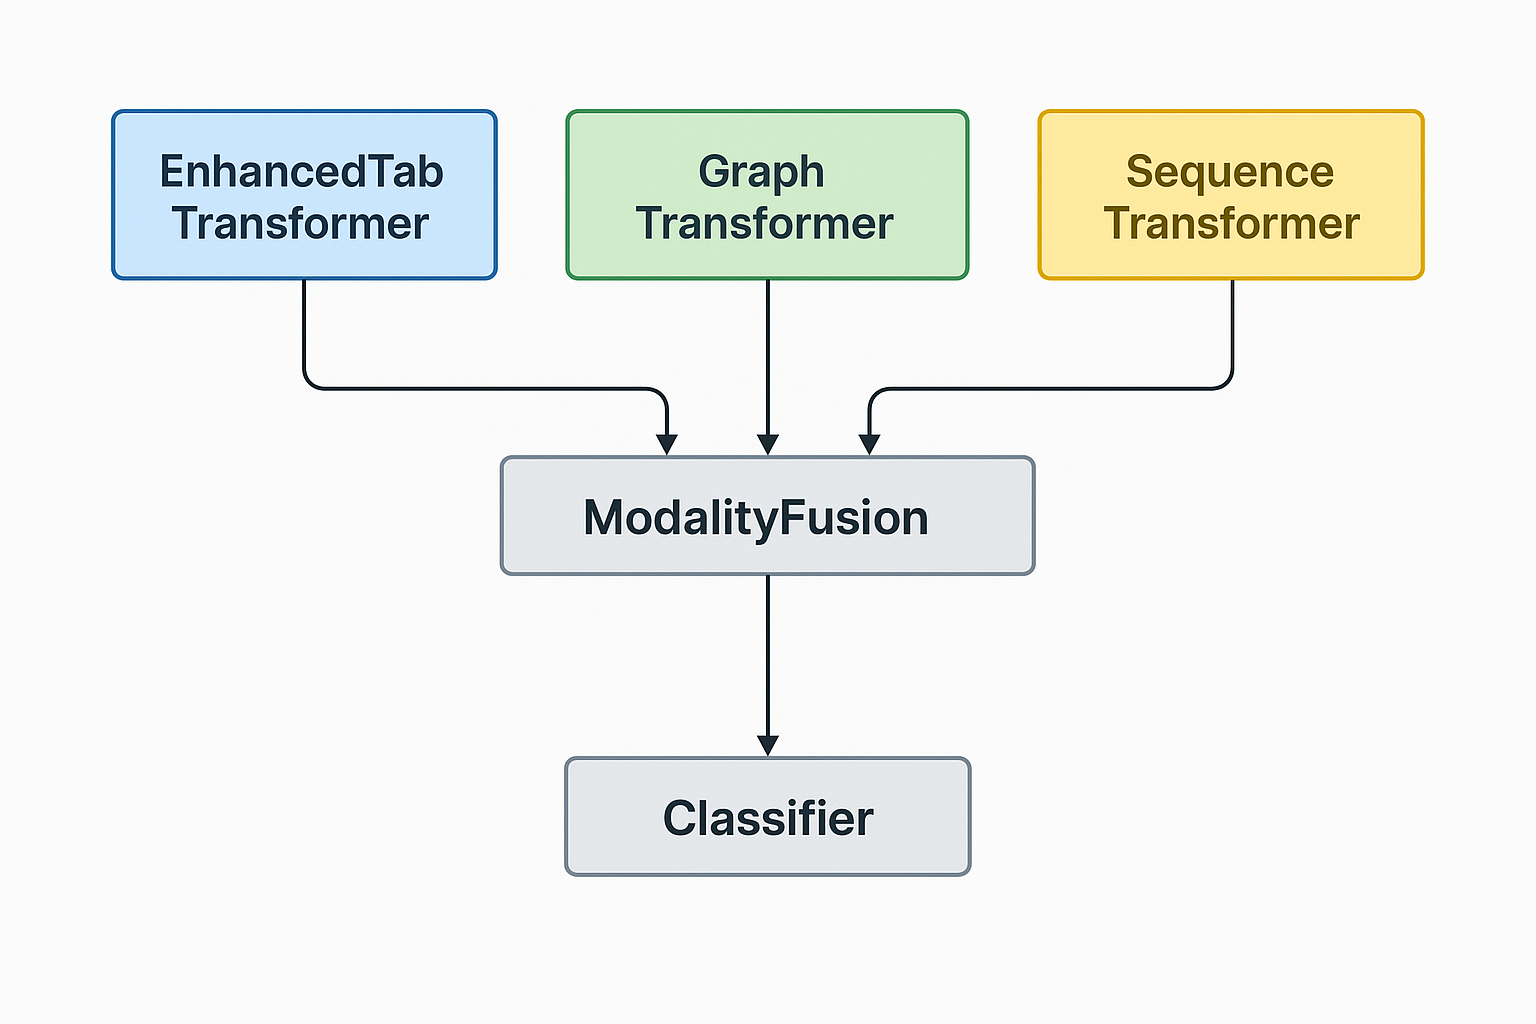
\includegraphics[width=0.9\textwidth]{../images/magnet_architecture.png}
\caption{معماری کلی مدل MAGNET}
\label{fig:magnet_architecture}
\end{figure}

\textbf{ماژول ویژگی‌های جدولی (EnhancedTabTransformer):}
این ماژول برای پردازش ویژگی‌های ایستا طراحی شده است. ویژگی‌های ورودی شامل:
\begin{itemize}
  \item مجوزهای درخواست‌شده توسط برنامه (\lr{128} ویژگی)
  \item اجزای برنامه مانند \lr{Activities}، \lr{Services}، و \lr{Receivers}
  \item فراخوانی‌های \lr{API} ایستا
  \item اطلاعات \lr{AndroidManifest.xml}
\end{itemize}

\begin{algorithm}[!htbp]
\caption{EnhancedTabTransformer Module Structure}
\label{alg:enhanced_tab_transformer}
\begin{algorithmic}[1]
\STATE \textbf{Input:} $x$ (tabular feature vector with dimensions $batch\_size \times input\_dim$)
\STATE Embed each feature using Linear layer, LayerNorm, and ReLU
\STATE Add positional embedding to each feature
\FOR{each transformer layer}
    \STATE Apply transformer layer on feature vectors
\ENDFOR
\STATE \textbf{Output:} Final feature vector
\end{algorithmic}
\end{algorithm}

\textbf{ماژول ساختار گراف (GraphTransformer):}
این ماژول برای تحلیل گراف‌های فراخوانی توابع طراحی شده است. گراف‌های ورودی دارای مشخصات زیر هستند:
\begin{itemize}
  \item میانگین \lr{1,245} گره و \lr{3,872} یال در هر نمونه
  \item ویژگی‌های گره: نوع تابع، فراوانی فراخوانی (\lr{64} بعد)
  \item ویژگی‌های یال: فراوانی و نوع فراخوانی (\lr{32} بعد)
\end{itemize}

\begin{algorithm}[!htbp]
\caption{GraphTransformer Module Structure}
\label{alg:graph_transformer}
\begin{algorithmic}[1]
\STATE \textbf{Input:} $data$ (containing $x$, $edge\_index$, $edge\_attr$)
\STATE Embed node features using Linear layer
\IF{edge features exist}
    \STATE Embed edge features using Linear layer
\ENDIF
\FOR{each graph transformer layer}
    \STATE Apply TransformerConv on nodes and edges
\ENDFOR
\STATE Apply global\_mean\_pool on nodes
\STATE \textbf{Output:} Graph feature vector
\end{algorithmic}
\end{algorithm}

\textbf{ماژول توالی‌های API (SequenceTransformer):}
این ماژول برای تحلیل توالی‌های فراخوانی \lr{API} طراحی شده است:
\begin{itemize}
  \item میانگین طول \lr{87} فراخوانی \lr{API} در هر نمونه
  \item رمزگذاری توالی‌ها با استفاده از \lr{Word2Vec}
  \item حفظ اطلاعات ترتیب زمانی فراخوانی‌ها
\end{itemize}

\begin{algorithm}[!htbp]
\caption{SequenceTransformer Module Structure}
\label{alg:sequence_transformer}
\begin{algorithmic}[1]
\STATE \textbf{Input:} $seq$ (sequence of API tokens)
\STATE Embed tokens using Embedding layer
\STATE Add positional encoding to sequence
\FOR{each transformer layer}
    \STATE Apply transformer layer on sequence
\ENDFOR
\STATE Calculate mean of vectors across sequence length
\STATE \textbf{Output:} Sequence feature vector
\end{algorithmic}
\end{algorithm}

\subsection{جزئیات پیاده‌سازی}
\textbf{مکانیزم توجه پویا:}
برای ادغام اطلاعات سه ماژول، مکانیزم توجه پویای زیر طراحی شده است:
\begin{equation}
\text{Attention}(Q, K, V) = \text{softmax}\left(\frac{QK^T}{\sqrt{d_k}}\right)V
\end{equation}

\begin{algorithm}[!htbp]
\caption{Dynamic Attention Mechanism}
\label{alg:dynamic_attention}
\begin{algorithmic}[1]
\STATE \textbf{Input:} $x$ (input vectors)
\STATE Calculate multi-head attention on $x$
\STATE Multiply output by learnable parameter $\gamma$
\STATE \textbf{Output:} Attended vectors and attention weights
\end{algorithmic}
\end{algorithm}
که در آن $Q$، $K$، و $V$ به ترتیب ماتریس‌های \lr{Query}، \lr{Key}، و \lr{Value} هستند.

\textbf{لایه ادغام چندوجهی:}
خروجی نهایی از طریق ترکیب وزنی خروجی‌های سه ماژول محاسبه می‌شود:
\begin{equation}
\text{Output} = \alpha \cdot h_{\text{tab}} + \beta \cdot h_{\text{graph}} + \gamma \cdot h_{\text{seq}}
\end{equation}

\begin{algorithm}[!htbp]
\caption{Modality Fusion}
\label{alg:modality_fusion}
\begin{algorithmic}[1]
\STATE \textbf{Input:} Outputs from three modules (tabular, graph, sequential)
\STATE Calculate mean of each output
\STATE Stack outputs into a matrix
\STATE Apply dynamic attention mechanism on output matrix
\STATE Calculate final mean
\STATE \textbf{Output:} Fused vector
\end{algorithmic}
\end{algorithm}
که وزن‌های $\alpha$، $\beta$، و $\gamma$ به صورت تطبیقی یاد گرفته می‌شوند.

\begin{algorithm}[!htbp]
\caption{Final MAGNET Model}
\label{alg:final_magnet}
\begin{algorithmic}[1]
\STATE \textbf{Input:} Tabular data, Graph data, Sequential data
\STATE Extract tabular features using EnhancedTabTransformer
\STATE Extract graph features using GraphTransformer
\STATE Extract sequential features using SequenceTransformer
\STATE Fuse three feature vectors using ModalityFusion
\STATE Apply final classifier (Fully Connected layers and Sigmoid)
\STATE \textbf{Output:} Probability of sample being malware
\end{algorithmic}
\end{algorithm}

\section{پیاده‌سازی و ارزیابی}
\subsection{مجموعه داده}
برای ارزیابی مدل \lr{MAGNET} از مجموعه داده استاندارد \lr{DREBIN}~\cite{Drebin} استفاده شد که شامل \lr{6,092} نمونه است:
\begin{itemize}
  \item \textbf{lu آموزش:} \lr{4,641} نمونه
  \item \textbf{تست:} \lr{1,451} نمونه (\lr{327} نمونه سالم، \lr{1,124} نمونه بدافزار)
  \item \textbf{دوره زمانی:} \lr{2010-2014}
  \item \textbf{خانواده‌های بدافزار:} شامل انواع مختلف بدافزار
\end{itemize}

\subsection{تنظیمات آزمایش}
\textbf{سخت‌افزار:}
\begin{itemize}
  \item \lr{CPU: Intel Core i7-8700K}
  \item \lr{GPU: NVIDIA RTX 3080} (10GB VRAM)
  \item \lr{RAM: 32GB DDR4-3200}
  \item \lr{Storage: 256GB NVMe SSD}
\end{itemize}

\textbf{نرم‌افزار:}
\begin{itemize}
  \item \lr{Python 3.8.10}
  \item \lr{PyTorch 1.12.0}
  \item \lr{PyTorch Geometric 2.1.0}
  \item \lr{CUDA 11.6}
\end{itemize}

\textbf{بهینه‌سازی پارامترها:}
بهینه‌سازی ابرپارامترها با دو روش انجام شد:
\begin{itemize}
  \item \textbf{بهینه‌سازی دستی:} الگوریتم \lr{PIRATES} با \lr{476} آزمایش
  \item \textbf{بهینه‌سازی \lr{Optuna}:} \lr{13} آزمایش هدفمند
\end{itemize}


\section{نتایج}
\subsection{عملکرد کلی}
مدل \lr{MAGNET} در ارزیابی بر روی مجموعه تست شامل \lr{1,451} نمونه به نتایج زیر دست یافت:
\begin{itemize}
    \item \textbf{دقت:} \lr{97.24\%}
    \item \textbf{\lr{F1-Score}:} \lr{0.9823}
    \item \textbf{\lr{Precision}:} \lr{0.9796}
    \item \textbf{\lr{Recall}:} \lr{0.9849}
    \item \textbf{\lr{AUC}:} \lr{0.9932}
\end{itemize}

\subsection{نتایج اعتبارسنجی متقاطع}
در اعتبارسنجی متقاطع \lr{5}-تایی، میانگین معیارها به صورت زیر به‌دست آمد:
\begin{table*}
  \centering
  \caption{نتایج اعتبارسنجی متقاطع \lr{5}-تایی مدل \lr{MAGNET}}
  \begin{tabular}{|l|c|}
    \hline
    \textbf{معیار} & \textbf{مقدار} \\
    \hline
    \hline
    دقت & \lr{0.9722 ± 0.0065} \\
    \hline
    \lr{Precision} & \lr{0.9810 ± 0.0102} \\
    \hline
    \lr{Recall} & \lr{0.9828 ± 0.0072} \\
    \hline
    \lr{F1-Score} & \lr{0.9818 ± 0.0042} \\
    \hline
    \lr{AUC} & \lr{0.9932 ± 0.0035} \\
  \end{tabular}
\end{table*}

\subsection{مقایسه با روش‌های مرجع}
\begin{table*}
  \centering
    \caption{مقایسه عملکرد مدل \lr{MAGNET} با روش‌های مرجع}
  \begin{tabular}{|l|c|c|c|c|c|}
    \hline
    \textbf{روش} & \textbf{دقت} & \textbf{\lr{F1-Priceision}} & \textbf{\lr{Recall}} & \textbf{\lr{F1-Score}} & \textbf{\lr{AUC}} \\
    \hline
    \lr{SVM} & \lr{0.906} & \lr{0.915} & \lr{0.892} & \lr{0.903} & \lr{0.945} \\
    \hline
    \lr{Random Forest} & \lr{0.935} & \lr{0.942} & \lr{0.928} & \lr{0.935} & \lr{0.967} \\
    \hline
    \lr{XGBoost} & \lr{0.948} & \lr{0.953} & \lr{0.943} & \lr{0.948} & \lr{0.978} \\
    \hline
    \lr{ANN} & \lr{0.962} & \lr{0.965} & \lr{0.959} & \lr{0.962} & \lr{0.985} \\
    \hline
    \textbf{\lr{MAGNET}} & \textbf{\lr{0.972}} & \textbf{\lr{0.980}} & \textbf{\lr{0.985}} & \textbf{\lr{0.982}} & \textbf{\lr{0.993}} \\
    \hline
  \end{tabular}
\end{table*}

\subsection{تحلیل عملکرد ماژول‌ها}
عملکرد تک‌تک ماژول‌های مدل \lr{MAGNET} بر اساس نتایج پایان‌نامه:
\begin{itemize}
    \item \textbf{\lr{EnhancedTabTransformer}} \lr{F1-Score = 0.945}
    \item \textbf{\lr{GraphTransformer}} \lr{F1-Score = 0.894}
    \item \textbf{\lr{SequenceTransformer}} \lr{F1-Score = 0.907}
    \item \textbf{مدل ترکیبی:} \lr{F1-Score = 0.982}
\end{itemize}

\subsection{مطالعه حذف اجزا (Ablation Study)}
بر اساس مطالعه حذف اجزا انجام‌شده در پایان‌نامه:
\begin{itemize}
  \item \textbf{بدون مکانیزم توجه پویا:} \lr{F1-Score = 0.954}
  \item \textbf{بدون لایه ادغام چندوجهی:} \lr{F1-Score = 0.967}
  \item \textbf{مدل کامل \lr{MAGNET}} \lr{F1-Score = 0.982}
\end{itemize}

\subsection{ماتریس درهم‌ریختگی}
نتایج تست نهایی بر روی \lr{1,451} نمونه تست:
\begin{itemize}
    \item \textbf{درست منفی (\lr{TN})}: \lr{304} نمونه
    \item \textbf{نادرست مثبت (\lr{FP})}: \lr{23} نمونه
    \item \textbf{نادرست منفی (\lr{FN})}: \lr{17} نمونه
    \item \textbf{درست مثبت (\lr{TP})}: \lr{1,107} نمونه
\end{itemize}

\subsection{مقایسه با روش‌های پیشرفته}
\begin{table*}
  \centering
  \caption{مقایسه با روش‌های پیشرفته}
  \begin{tabular}{|l|c|c|c|c|}
    \hline
    \textbf{روش} & \textbf{دقت (\%)} & \textbf{\lr{F1-Score}} & \textbf{\lr{AUC}} & \textbf{یادداشت} \\
    \hline
    \textbf{\lr{MAGNET}} & \textbf{\lr{97.24}} & \textbf{\lr{0.9823}} & \textbf{\lr{0.9932}} & بهترین عملکرد، \lr{DREBIN} \\
    \hline
    \lr{DREBIN} (\lr{SVM}) & \lr{92.3} & \lr{0.933} & \lr{0.955} & رویکرد ایستا \\
    \hline
    \lr{PIKADROID} & \lr{96.8} & \lr{0.974} & \lr{0.988} & تحلیل \lr{API}، \lr{DREBIN} \\
    \hline
    \lr{CrossMalDroid} & \lr{95.2} & \lr{0.952} & \lr{0.976} & انتخاب ویژگی، \lr{Malgenome} \\
    \hline
    \lr{DroidAPIMiner} & \lr{89.7} & \lr{0.891} & \lr{0.927} & فرکانس \lr{API}، \lr{DREBIN} \\
    \hline
    \lr{DeepImageDroid} & \lr{96.0} & \lr{0.960} & \lr{0.982} & ترنسفورمر بصری و \lr{CNN} \\
    \hline
    \lr{BERT-Graph} & \lr{95.5} & \lr{0.950} & \lr{0.975} & \lr{BERT} و گراف \lr{API} \\
  \hline
\end{tabular}
\end{table*}

\begin{figure}[!htbp]
\centering

\includegraphics[width=0.9\textwidth]{../images/fig_literature_comparison.png}
\caption{مقایسه عملکرد مدل MAGNET با روش‌های پیشرفته}
\label{fig:literature_comparison}
\end{figure}

\section{بحث و تحلیل}
\subsection{تحلیل نتایج}
نتایج به‌دست آمده نشان می‌دهد که مدل \lr{MAGNET} با دقت \lr{97.24\%} و \lr{F1-Score} برابر \lr{0.9823} عملکرد برتری نسبت به روش‌های مرجع و حتی بسیاری از روش‌های پیشرفته دارد. این بهبود عملکرد را می‌توان به عوامل زیر نسبت داد:
\textbf{تنوع اطلاعات:}
استفاده از سه نوع داده مختلف (جدولی، گرافی، ترتیبی) اطلاعات جامع‌تری از ساختار و رفتار برنامه‌ها فراهم می‌کند.
\textbf{معماری پیشرفته:}
استفاده از ترنسفورمرهای تخصصی امکان استخراج الگوهای پیچیده را فراهم می‌کند.
\textbf{مکانیزم توجه پویا:}
این مکانیزم امکان تمرکز بر اطلاعات مهم و نادیده گرفتن اطلاعات نامربوط را فراهم می‌کند.

\subsection{مقایسه با کارهای پیشین}
در مقایسه با کارهای پیشین:
\begin{itemize}
    \item \textbf{\lr{DREBIN} اصلی:} دقت \lr{94}\% - بهبود \lr{3.24}\%
    \item \textbf{روش‌های چندوجهی قبلی:} دقت حدود \lr{89-96}\% - بهبود قابل‌توجه
    \item \textbf{روش‌های مبتنی بر \lr{GNN}:} دقت حدود \lr{95-97}\% - رقابتی یا بهتر
\end{itemize}

\subsection{محدودیت‌ها}
علی‌رغم نتایج مثبت، مدل \lr{MAGNET} دارای محدودیت‌هایی است:
\textbf{پیچیدگی محاسباتی:}
پردازش سه نوع داده مختلف نیازمند منابع قابل‌توجه است.
\textbf{وابستگی به کیفیت داده:}
عملکرد مدل به کیفیت استخراج ویژگی و پیش‌پردازش داده‌ها وابسته است.
\textbf{تعمیمی‌پذیری:}
آموزش بر روی مجموعه داده \lr{DREBIN} که مربوط به سال‌های \lr{2010-2014} است، ممکن است تعمیم‌پذیری مدل را محدود کند.

\section{نتیجه‌گیری}
این پژوهش مدل نوآورانه \lr{MAGNET} را برای تشخیص بدافزار اندروید معرفی کرد که از رویکرد چندوجهی و معماری‌های پیشرفته استفاده می‌کند. نتایج ارزیابی بر روی مجموعه داده \lr{DREBIN} نشان می‌دهد که با دقت \lr{97.24\%} و \lr{F1-Score} برابر \lr{0.9823} عملکرد برتری نسبت به روش‌ها دارد.

دستاوردهای کلیدی عبارتند از:
\begin{itemize}
    \item طراحی معماری چندوجهی یکپارچه با سه ماژول تخصصی شامل \lr{EnhancedTabTransformer}، \lr{GraphTransformer}، و \lr{SequenceTransformer}
    \item توسعه مکانیزم توجه پویا برای ادغام بهینه اطلاعات با وزن‌های تطبیقی
    \item نشان دادن اهمیت استفاده از اطلاعات متنوع شامل ویژگی‌های جدولی، گرافی و ترتیبی
    \item ارائه راه‌حلی عملی برای سیستم‌های امنیتی با دقت بالا و نرخ خطای پایین
    \item استفاده موثر از از الگوریتم بهینه‌سازی \lr{PIRATES} برای تنظیم خودکار
\end{itemize}

مطالعه حذف اجزا تأیید کرد که هر ماژول نقش مهمی دارد و حذف آن‌ها منجر به کاهش دقت می‌شود. ماتریس درهم‌ریختگی نشان داد توانایی در تفکیک صحیح نمونه‌های مخرب و سالم دارد.

\section{پیشنهادات آتی}
\subsection{بهبودهای فنی}
\begin{itemize}
    \item ارزیابی مدل بر روی مجموعه داده‌های جدیدتر و متنوع‌تر شامل بدافزارهای سال‌های اخیر
    \item بهینه‌سازی معماری برای کاهش پیچیدگی محاسباتی و افزایش سرعت پردازش
    \item توسعه تکنیک‌های فشرده‌سازی مدل برای اجرا بر روی دستگاه‌های با منابع محدود
    \item پیاده‌سازی یادگیری انتقالی برای تطبیق سریع با انواع جدید بدافزار
\end{itemize}

\subsection{کاربردهای عملی}
\begin{itemize}
    \item بررسی قابلیت اعمال مدل در محیط‌های عملیاتی و سیستم‌های تولیدی
    \item توسعه رابط کاربری برای استفاده آسان توسط متخصصان امنیت
    \item ادغام مدل با سیستم‌های موجود آنتی‌ویروس و امنیتی
    \item بررسی عملکرد مدل در تشخیص \textit{real-time} بدافزارها
\end{itemize}

\subsection{تحقیقات آینده}
\begin{itemize}
    \item توسعه روش‌های تفسیرپذیری برای درک بهتر فرآیند تصمیم‌گیری مدل
    \item بررسی مقاومت مدل در برابر حملات تضاد و تکنیک‌های فرار پیشرفته
    \item توسعه مدل‌های تطبیقی که بتوانند با تکامل بدافزارها به‌روزرسانی شوند
    \item بررسی کاربرد مدل برای تشخیص انواع دیگر نرم‌افزارهای مخرب در پلتفرم‌های مختلف
\end{itemize}

\newpage
\begin{latin}
  \printbibliography[heading=bibintoc,title={مراجع}]
\end{latin}

% چکیده انگلیسی
\newpage
\begin{latin}
\section*{\fontsize{16}{17}\selectfont \bfseries Abstract}
\setlength{\parindent}{0pt}\fontsize{12}{13}\selectfont
Android malware detection is becoming a major challenge in information security due to the increasing cyber threats. Traditional methods, especially those relying solely on single-modal feature analysis, often face limitations such as the inability to process complex multi-modal data and poor generalization to new threats. These shortcomings highlight the need for developing novel and efficient approaches. This research proposes a multi-modal model called Multi-modal Attention-based Graph Neural Transformer with Dynamic Embedding (MAGNET), which leverages a combination of tabular, graph, and sequential data—such as API call sequences—for Android malware detection. The primary objective is to improve detection accuracy and robustness by utilizing an advanced architecture based on deep learning and transformers. The methodology includes hyperparameter optimization using advanced algorithms such as PIRATES and Optuna, along with model training on a dataset consisting of 4641 training samples and 1451 test samples, supported by 5-fold cross-validation. The model incorporates static features such as permissions, API calls, intents, and component names, as well as dynamic features like network activity and file access. Data is represented as binary or normalized numerical vectors, and the feature space is reduced to 430 dimensions after preprocessing. Tools used in this study include deep learning libraries such as PyTorch, data preprocessing techniques like standardization and normalization, and graph data structures. The raw data consists of actual Android application behavior, encompassing both static and dynamic attributes. Results indicate that the proposed model delivers outstanding performance with high accuracy, notable stability, and strong generalization, offering significant improvements over previous methods. These outcomes underscore the model's potential for deployment in real-world security systems.

\par\vspace{.5cm}\setlength{\parindent}{0pt}
{\fontsize{13}{14}\selectfont\bfseries Keywords: Malware Detection, Transformer, Deep Learning, Multi-modal Data, Android Security.}
\end{latin}

\cleardoublepage

% کاور انگلیسی
\begin{latin}
\thispagestyle{empty}
\setlength{\parindent}{0pt}
\begin{center}

\includegraphics[height=2cm]{logo} \\[0.3cm]
{\fontsize{14}{15}\selectfont \textbf{Shahid Bahonar University of Kerman}} \\[0.2cm]
{\fontsize{14}{15}\selectfont\textbf{Faculty of  Engineering }} \\[0.2cm]
{\fontsize{14}{15}\selectfont\textbf{Department of Computer Engineering}} \\[1cm]

\hrule height 2pt
\vskip 0.5cm
{\fontsize{16}{17}\selectfont\bfseries
Robust Android Malware Detection using Transformer Neural\\
 Networks}
\vskip 0.5cm
\hrule height 2pt

\vskip 2cm
{\fontsize{16}{17}\selectfont \bfseries
Prepared by:} \\[0.3cm]
{\fontsize{14}{15}\selectfont \bfseries
Alireza Iranmanesh}

\vskip 1cm
{\fontsize{16}{17}\selectfont \bfseries
Supervisor:} \\[0.3cm]
{\fontsize{14}{15}\selectfont \bfseries
Dr. Hamid Mirvaziri}

\vskip 2cm
{\fontsize{14}{15}\selectfont \bfseries
A Thesis Submitted as a Partial Fulfillment of the Requirements for the \\
Degree of Master of Science in Computer Engineering (M. Sc.)}

\vskip 1.5cm
{\fontsize{14}{15}\selectfont \bfseries
June 2025}
\end{center}
\end{latin}

\end{document}